

\tikzset{every picture/.style={line width=0.75pt}} %set default line width to 0.75pt

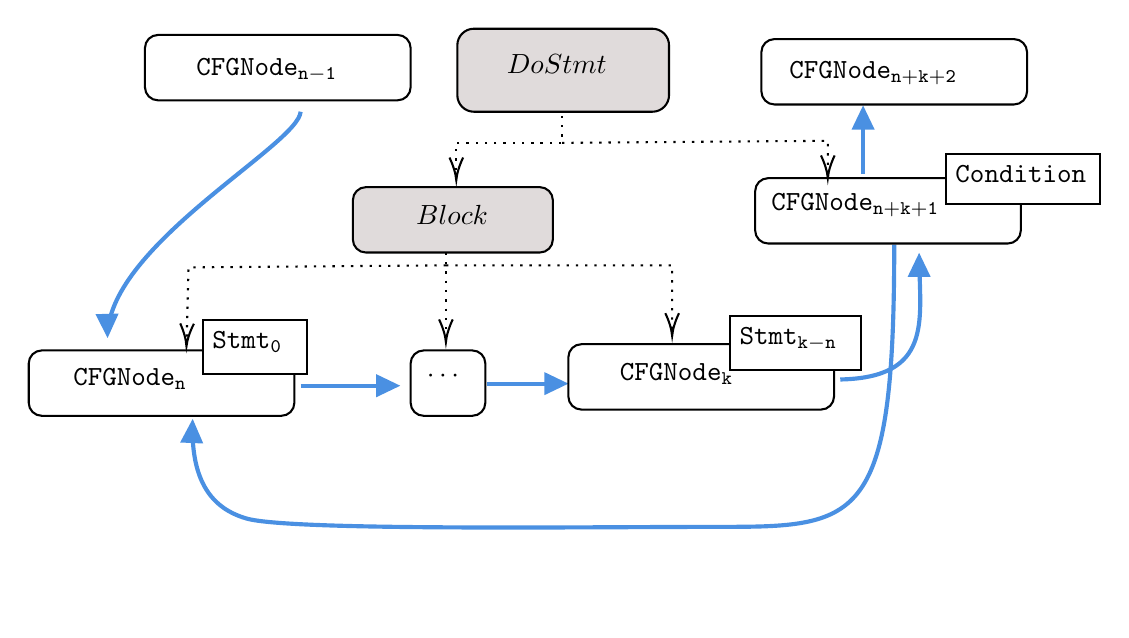
\begin{tikzpicture}[x=0.75pt,y=0.75pt,yscale=-1,xscale=1]
%uncomment if require: \path (0,607); %set diagram left start at 0, and has height of 607

%Rounded Rect [id:dp4103371580938808]
\draw  [color={rgb, 255:red, 0; green, 0; blue, 0 }  ,draw opacity=1 ][fill={rgb, 255:red, 224; green, 219; blue, 219 }  ,fill opacity=1 ] (502.5,104) .. controls (502.5,99.58) and (506.08,96) .. (510.5,96) -- (596.5,96) .. controls (600.92,96) and (604.5,99.58) .. (604.5,104) -- (604.5,128) .. controls (604.5,132.42) and (600.92,136) .. (596.5,136) -- (510.5,136) .. controls (506.08,136) and (502.5,132.42) .. (502.5,128) -- cycle ;
%Rounded Rect [id:dp7186258831078288]
\draw   (352,105.3) .. controls (352,101.82) and (354.82,99) .. (358.3,99) -- (473.7,99) .. controls (477.18,99) and (480,101.82) .. (480,105.3) -- (480,124.2) .. controls (480,127.68) and (477.18,130.5) .. (473.7,130.5) -- (358.3,130.5) .. controls (354.82,130.5) and (352,127.68) .. (352,124.2) -- cycle ;
%Curve Lines [id:da5255003767655927]
\draw [color={rgb, 255:red, 74; green, 144; blue, 226 }  ,draw opacity=1 ][line width=1.5]    (427,136) .. controls (426.03,151.52) and (338.5,198.09) .. (334.16,241.03) ;
\draw [shift={(334,245)}, rotate = 268.7] [fill={rgb, 255:red, 74; green, 144; blue, 226 }  ,fill opacity=1 ][line width=0.08]  [draw opacity=0] (11.61,-5.58) -- (0,0) -- (11.61,5.58) -- cycle    ;
%Curve Lines [id:da7123104582514019]
\draw [color={rgb, 255:red, 74; green, 144; blue, 226 }  ,draw opacity=1 ][line width=1.5]    (713,200) .. controls (713,333) and (697,336) .. (631,336) .. controls (565,336) and (422,338) .. (401,332) .. controls (381.16,326.33) and (374.71,309.94) .. (374.9,287.9) ;
\draw [shift={(375,284)}, rotate = 452.39] [fill={rgb, 255:red, 74; green, 144; blue, 226 }  ,fill opacity=1 ][line width=0.08]  [draw opacity=0] (11.61,-5.58) -- (0,0) -- (11.61,5.58) -- cycle    ;
%Curve Lines [id:da25467631423079007]
\draw [color={rgb, 255:red, 74; green, 144; blue, 226 }  ,draw opacity=1 ][line width=1.5]    (725.04,208.17) .. controls (725.61,237.55) and (730.93,264.05) .. (687,265) ;
\draw [shift={(725,204)}, rotate = 90] [fill={rgb, 255:red, 74; green, 144; blue, 226 }  ,fill opacity=1 ][line width=0.08]  [draw opacity=0] (11.61,-5.58) -- (0,0) -- (11.61,5.58) -- cycle    ;
%Rounded Rect [id:dp9303397570251196]
\draw  [fill={rgb, 255:red, 224; green, 219; blue, 219 }  ,fill opacity=1 ] (452.17,178.63) .. controls (452.17,175.15) and (454.99,172.33) .. (458.47,172.33) -- (542.23,172.33) .. controls (545.71,172.33) and (548.53,175.15) .. (548.53,178.63) -- (548.53,197.53) .. controls (548.53,201.01) and (545.71,203.83) .. (542.23,203.83) -- (458.47,203.83) .. controls (454.99,203.83) and (452.17,201.01) .. (452.17,197.53) -- cycle ;
%Straight Lines [id:da5458056196073965]
\draw [color={rgb, 255:red, 74; green, 144; blue, 226 }  ,draw opacity=1 ][line width=1.5]    (427,268) -- (471,268) ;
\draw [shift={(475,268)}, rotate = 180] [fill={rgb, 255:red, 74; green, 144; blue, 226 }  ,fill opacity=1 ][line width=0.08]  [draw opacity=0] (11.61,-5.58) -- (0,0) -- (11.61,5.58) -- cycle    ;
%Straight Lines [id:da1567518694917287]
\draw [color={rgb, 255:red, 74; green, 144; blue, 226 }  ,draw opacity=1 ][line width=1.5]    (517,267) -- (552,267) ;
\draw [shift={(556,267)}, rotate = 180] [fill={rgb, 255:red, 74; green, 144; blue, 226 }  ,fill opacity=1 ][line width=0.08]  [draw opacity=0] (11.61,-5.58) -- (0,0) -- (11.61,5.58) -- cycle    ;
%Straight Lines [id:da23667241111262138]
\draw [color={rgb, 255:red, 74; green, 144; blue, 226 }  ,draw opacity=1 ][line width=1.5]    (698,166) -- (698,137) ;
\draw [shift={(698,133)}, rotate = 450] [fill={rgb, 255:red, 74; green, 144; blue, 226 }  ,fill opacity=1 ][line width=0.08]  [draw opacity=0] (11.61,-5.58) -- (0,0) -- (11.61,5.58) -- cycle    ;
%Rounded Rect [id:dp9545385553768504]
\draw   (296,257.3) .. controls (296,253.82) and (298.82,251) .. (302.3,251) -- (417.7,251) .. controls (421.18,251) and (424,253.82) .. (424,257.3) -- (424,276.2) .. controls (424,279.68) and (421.18,282.5) .. (417.7,282.5) -- (302.3,282.5) .. controls (298.82,282.5) and (296,279.68) .. (296,276.2) -- cycle ;
%Rounded Rect [id:dp4665296267695891]
\draw   (480,257.3) .. controls (480,253.82) and (482.82,251) .. (486.3,251) -- (509.7,251) .. controls (513.18,251) and (516,253.82) .. (516,257.3) -- (516,276.2) .. controls (516,279.68) and (513.18,282.5) .. (509.7,282.5) -- (486.3,282.5) .. controls (482.82,282.5) and (480,279.68) .. (480,276.2) -- cycle ;
%Rounded Rect [id:dp31005795669558567]
\draw   (556,254.3) .. controls (556,250.82) and (558.82,248) .. (562.3,248) -- (677.7,248) .. controls (681.18,248) and (684,250.82) .. (684,254.3) -- (684,273.2) .. controls (684,276.68) and (681.18,279.5) .. (677.7,279.5) -- (562.3,279.5) .. controls (558.82,279.5) and (556,276.68) .. (556,273.2) -- cycle ;
%Rounded Rect [id:dp20286707122304926]
\draw   (646,174.3) .. controls (646,170.82) and (648.82,168) .. (652.3,168) -- (767.7,168) .. controls (771.18,168) and (774,170.82) .. (774,174.3) -- (774,193.2) .. controls (774,196.68) and (771.18,199.5) .. (767.7,199.5) -- (652.3,199.5) .. controls (648.82,199.5) and (646,196.68) .. (646,193.2) -- cycle ;
%Rounded Rect [id:dp34866856286152814]
\draw   (649,107.3) .. controls (649,103.82) and (651.82,101) .. (655.3,101) -- (770.7,101) .. controls (774.18,101) and (777,103.82) .. (777,107.3) -- (777,126.2) .. controls (777,129.68) and (774.18,132.5) .. (770.7,132.5) -- (655.3,132.5) .. controls (651.82,132.5) and (649,129.68) .. (649,126.2) -- cycle ;
%Straight Lines [id:da5919120314726174]
\draw  [dash pattern={on 0.84pt off 2.51pt}]  (497.05,210.01) -- (373,211) -- (372.05,247) ;
\draw [shift={(372,249)}, rotate = 271.51] [color={rgb, 255:red, 0; green, 0; blue, 0 }  ][line width=0.75]    (10.93,-3.29) .. controls (6.95,-1.4) and (3.31,-0.3) .. (0,0) .. controls (3.31,0.3) and (6.95,1.4) .. (10.93,3.29)   ;
%Straight Lines [id:da83242619742772]
\draw  [dash pattern={on 0.84pt off 2.51pt}]  (497.05,210.01) -- (606,210) -- (606,242) ;
\draw [shift={(606,244)}, rotate = 270] [color={rgb, 255:red, 0; green, 0; blue, 0 }  ][line width=0.75]    (10.93,-3.29) .. controls (6.95,-1.4) and (3.31,-0.3) .. (0,0) .. controls (3.31,0.3) and (6.95,1.4) .. (10.93,3.29)   ;
%Straight Lines [id:da23877345260011285]
\draw  [dash pattern={on 0.84pt off 2.51pt}]  (497,204) -- (497,245) ;
\draw [shift={(497,247)}, rotate = 270] [color={rgb, 255:red, 0; green, 0; blue, 0 }  ][line width=0.75]    (10.93,-3.29) .. controls (6.95,-1.4) and (3.31,-0.3) .. (0,0) .. controls (3.31,0.3) and (6.95,1.4) .. (10.93,3.29)   ;
%Straight Lines [id:da6580782336510713]
\draw  [dash pattern={on 0.84pt off 2.51pt}]  (553,138) -- (553,151) -- (502,151) -- (502,167) ;
\draw [shift={(502,169)}, rotate = 270] [color={rgb, 255:red, 0; green, 0; blue, 0 }  ][line width=0.75]    (10.93,-3.29) .. controls (6.95,-1.4) and (3.31,-0.3) .. (0,0) .. controls (3.31,0.3) and (6.95,1.4) .. (10.93,3.29)   ;
%Straight Lines [id:da6027446043982454]
\draw  [dash pattern={on 0.84pt off 2.51pt}]  (553,151) -- (681,150) -- (681,166) ;
\draw [shift={(681,168)}, rotate = 270] [color={rgb, 255:red, 0; green, 0; blue, 0 }  ][line width=0.75]    (10.93,-3.29) .. controls (6.95,-1.4) and (3.31,-0.3) .. (0,0) .. controls (3.31,0.3) and (6.95,1.4) .. (10.93,3.29)   ;

% Text Node
\draw (524.83,107) node [anchor=north west][inner sep=0.75pt]    {$DoStmt$};
% Text Node
\draw (375.3,109) node [anchor=north west][inner sep=0.75pt]    {$\mathtt{CFGNode_{n-1}}$};
% Text Node
\draw (661,110.3) node [anchor=north west][inner sep=0.75pt]    {$\mathtt{CFGNode_{n+k+2}}$};
% Text Node
\draw (652.3,174) node [anchor=north west][inner sep=0.75pt]    {$\mathtt{CFGNode_{n+k+1}}$};
% Text Node
\draw (481.17,179.63) node [anchor=north west][inner sep=0.75pt]    {$Block$};
% Text Node
\draw (316,258.3) node [anchor=north west][inner sep=0.75pt]    {$\mathtt{CFGNode_{n}}$};
% Text Node
\draw (486.3,259) node [anchor=north west][inner sep=0.75pt]    {$\cdots $};
% Text Node
\draw (579.3,256) node [anchor=north west][inner sep=0.75pt]    {$\mathtt{CFGNode_{k}}$};
% Text Node
\draw (504.17,373.63) node [anchor=north west][inner sep=0.75pt]    {$$};
% Text Node
\draw  [fill={rgb, 255:red, 255; green, 255; blue, 255 }  ,fill opacity=1 ]  (380,236.3) -- (430,236.3) -- (430,262.3) -- (380,262.3) -- cycle  ;
\draw (383,240.3) node [anchor=north west][inner sep=0.75pt]    {$\mathtt{Stmt_{0}}$};
% Text Node
\draw  [fill={rgb, 255:red, 255; green, 255; blue, 255 }  ,fill opacity=1 ]  (634,234.3) -- (697,234.3) -- (697,260.3) -- (634,260.3) -- cycle  ;
\draw (637,238.3) node [anchor=north west][inner sep=0.75pt]    {$\mathtt{Stmt_{k-n}}$};
% Text Node
\draw  [fill={rgb, 255:red, 255; green, 255; blue, 255 }  ,fill opacity=1 ]  (738,156.3) -- (812,156.3) -- (812,180.3) -- (738,180.3) -- cycle  ;
\draw (741,160.3) node [anchor=north west][inner sep=0.75pt]    {$\mathtt{Condition}$};


\end{tikzpicture}
